%================================================================
\section{Results and Discussion}\label{sec:Results}
%================================================================

%----------------------------------------------------------------
\subsection{Project Results 1}\label{sec:project results}
%----------------------------------------------------------------

%----------------------------------------------------------------
\subsection{Heat Equation}\label{sec:heateq results}
%----------------------------------------------------------------

\subsection{Forward Euler}
Nx = 11
Nt = 199

Max diff: 0.04009472326320718
Mean diff: 0.003186288853514369

\autoref{fig:heat_fe}
\begin{figure}[H]
\centering
\subfloat[]{{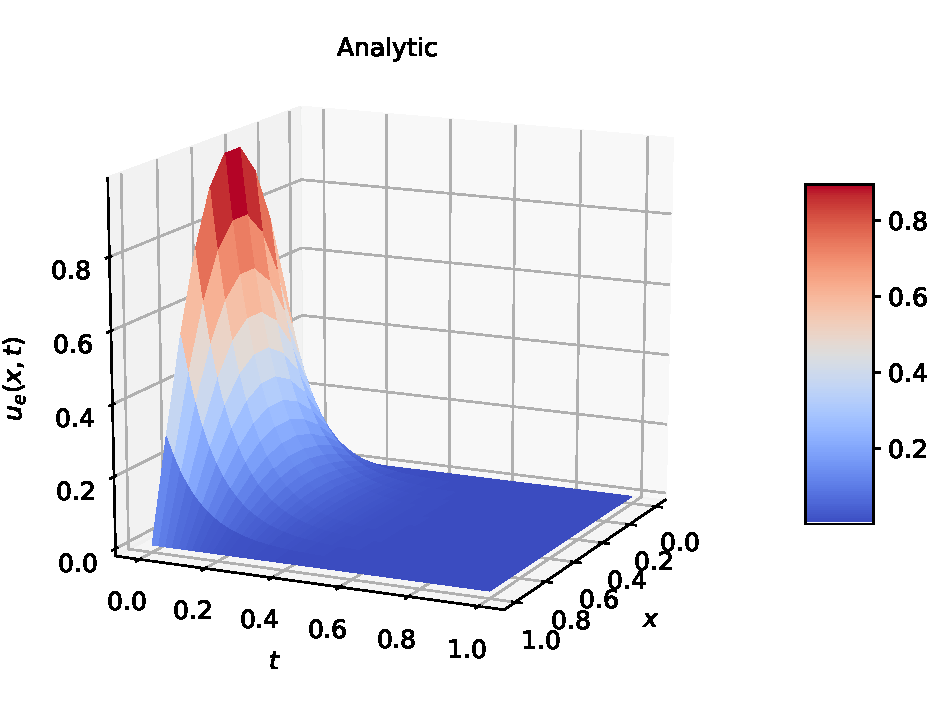
\includegraphics[scale=0.48]{latex/figures/heat_ana_fe.pdf}}}
\qquad
\subfloat[]{{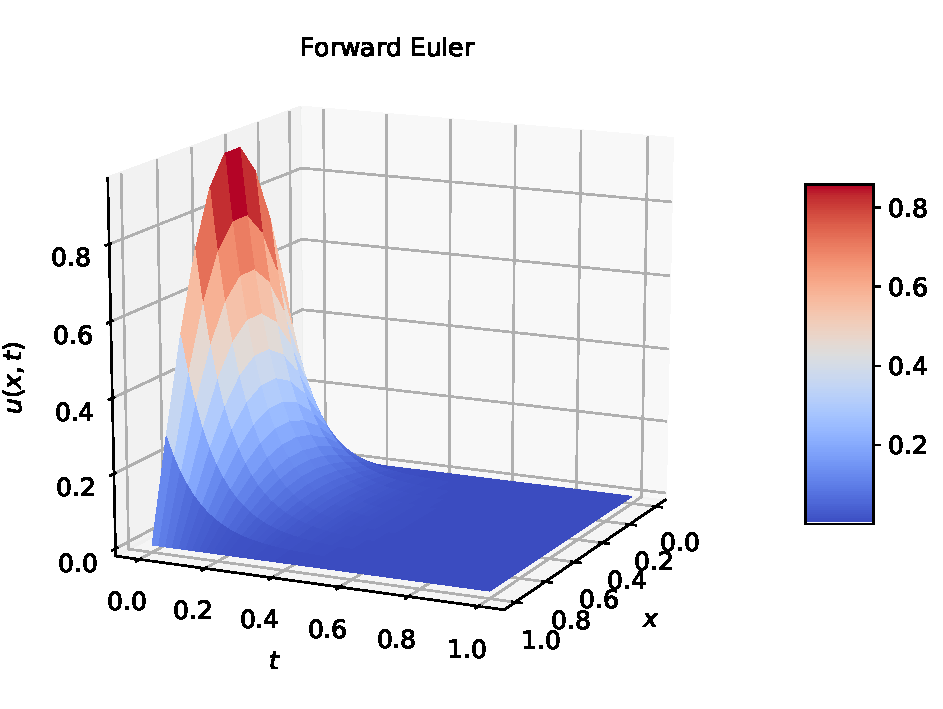
\includegraphics[scale=0.48]{latex/figures/heat_fe.pdf}}}
\qquad
\subfloat[]{{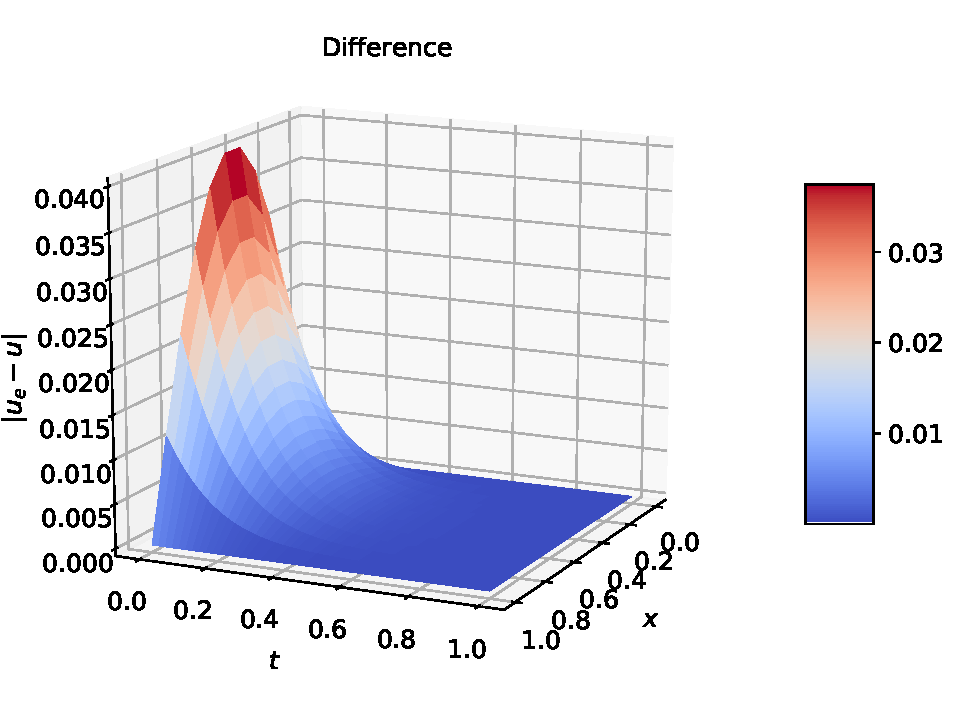
\includegraphics[scale=0.5]{latex/figures/heat_diff_fe.pdf}}}
\caption{FE heat}
\label{fig:heat_fe}
\end{figure}

CPU benchmark
Number of iterations: 1000
FE mean CPU time: 0.00158 secs


\subsubsection{FFNN}

\subsubsection{Model 1}
Model 1: Train on spatial and temporal points as dictated by FE stability criterion

Nx = 11
Nt = 199
2 layers + output, [150, 50, 1], [tanh, sigmoid, none] 
1000 epochs
Adam, initial lr=0.01
Step: 1000, Loss: 0.008064055285575904
Training FFNN CPU time: 147.62562 secs

\autoref{fig:heat_nn1} Plot solution on the grid FFNN is trained on

Max diff: 0.008466789818225778
Mean diff: 0.0029635112954797672

\begin{figure}[H]
\centering
\subfloat[]{{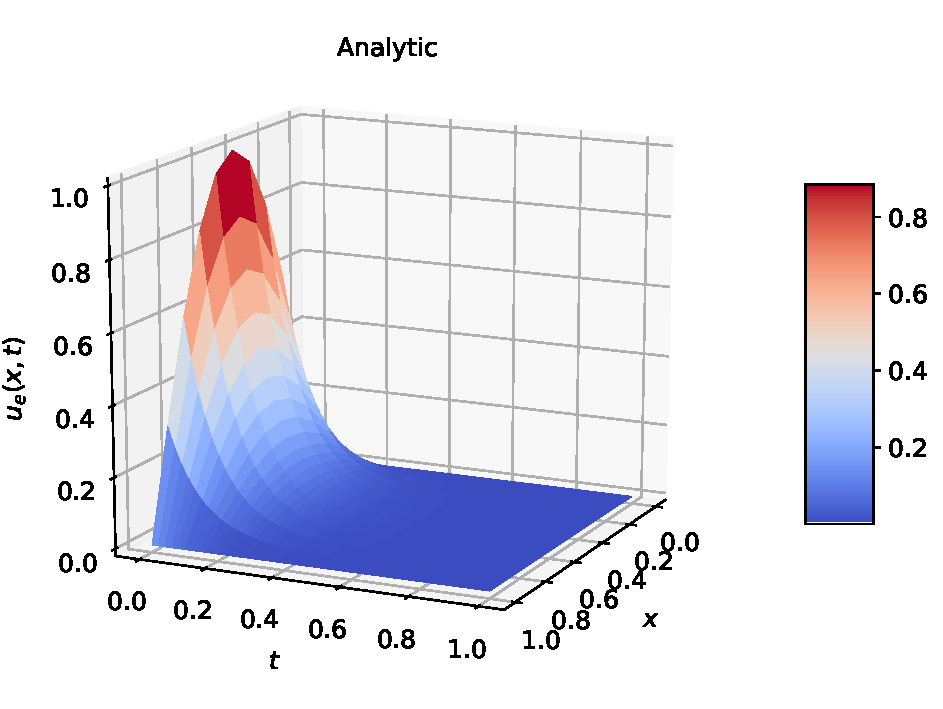
\includegraphics[scale=0.48]{latex/figures/heat_ana_nn1.pdf}}}
\qquad
\subfloat[]{{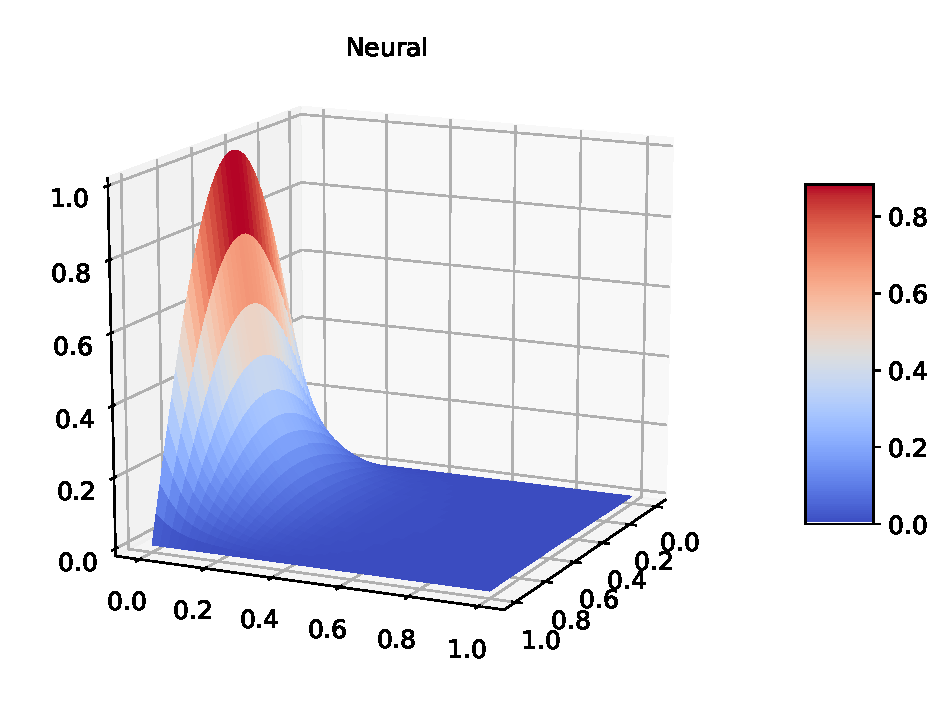
\includegraphics[scale=0.48]{latex/figures/heat_nn1.pdf}}}
\qquad
\subfloat[]{{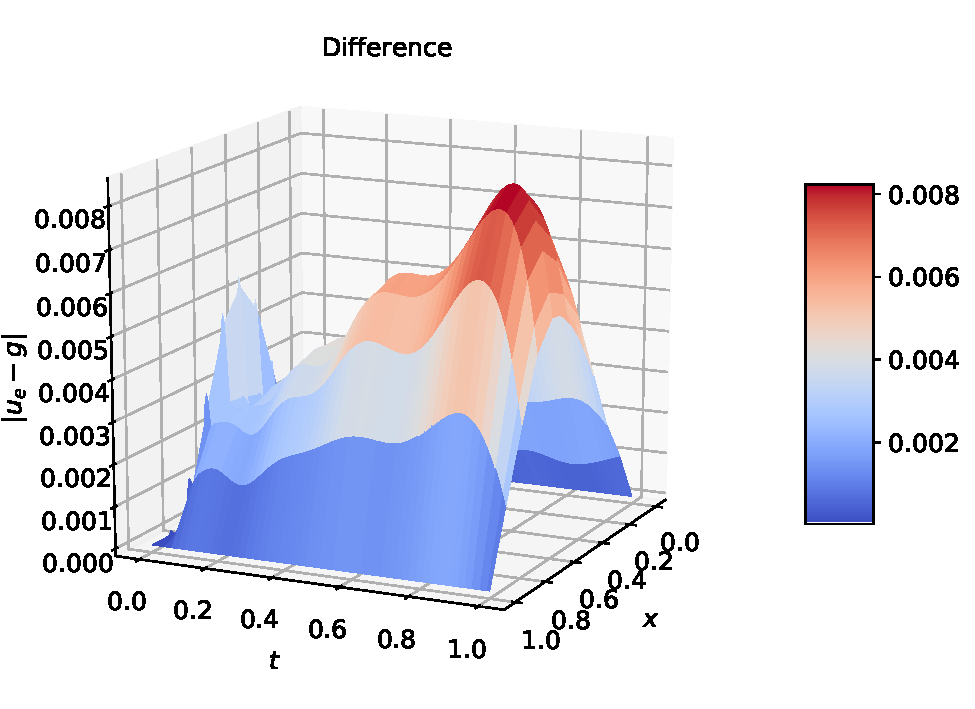
\includegraphics[scale=0.5]{latex/figures/heat_diff_nn1.pdf}}}
\caption{Model 1, Plot solution on the grid FFNN is trained on}
\label{fig:heat_nn1}
\end{figure}

\autoref{fig:heat_nn2} Plot solution on a larger grid than FFNN is trained on, i.e., points must be interpolated

301, 301 points

Max diff: 0.008467176325477247
Mean diff: 0.0032787069037113277

\begin{figure}[H]
\centering
\subfloat[]{{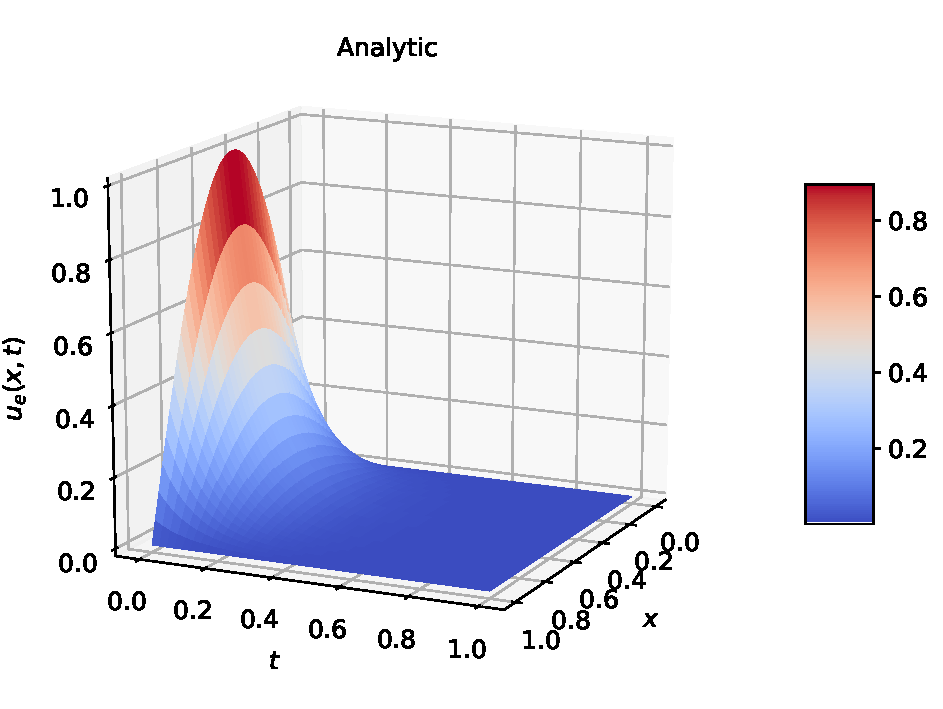
\includegraphics[scale=0.48]{latex/figures/heat_ana_nn2.pdf}}}
\qquad
\subfloat[]{{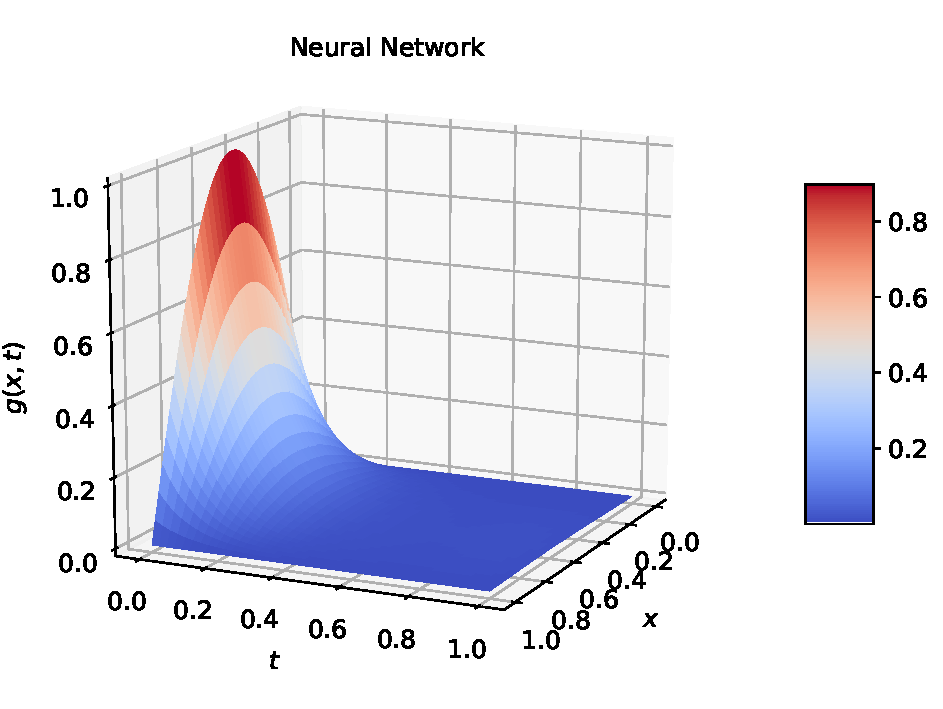
\includegraphics[scale=0.48]{latex/figures/heat_nn2.pdf}}}
\qquad
\subfloat[]{{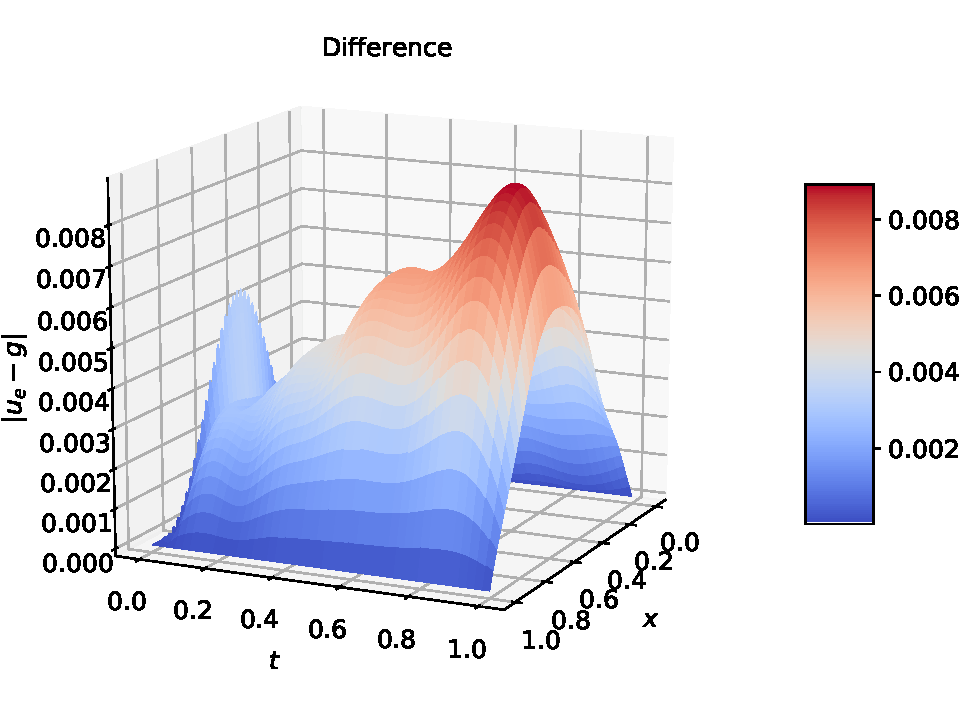
\includegraphics[scale=0.5]{latex/figures/heat_diff_nn2.pdf}}}
\caption{Model 1, Plot solution on a larger grid than FFNN is trained on, i.e., points must be interpolated}
\label{fig:heat_nn2}
\end{figure}

\subsubsection{Model 2}
Model 2: Train on equal number of spatial and temporal points

Nx = 11
Nt = 11
2 layers + output, [150, 50, 1], [tanh, sigmoid, none] 
1000 epochs
Adam, initial lr=0.01
Step: 1000, Loss: 0.008064055285575904
Training FFNN CPU time: 147.62562 secs
Step: 1000, Loss: 0.0027709536906761877
Training FFNN CPU time: 42.11612 secs

\autoref{fig:heat_nn3} Plot solution on the grid FFNN is trained on

Max diff: 0.026960711104318635
Mean diff: 0.0029851059330631173

\begin{figure}[H]
\centering
\subfloat[]{{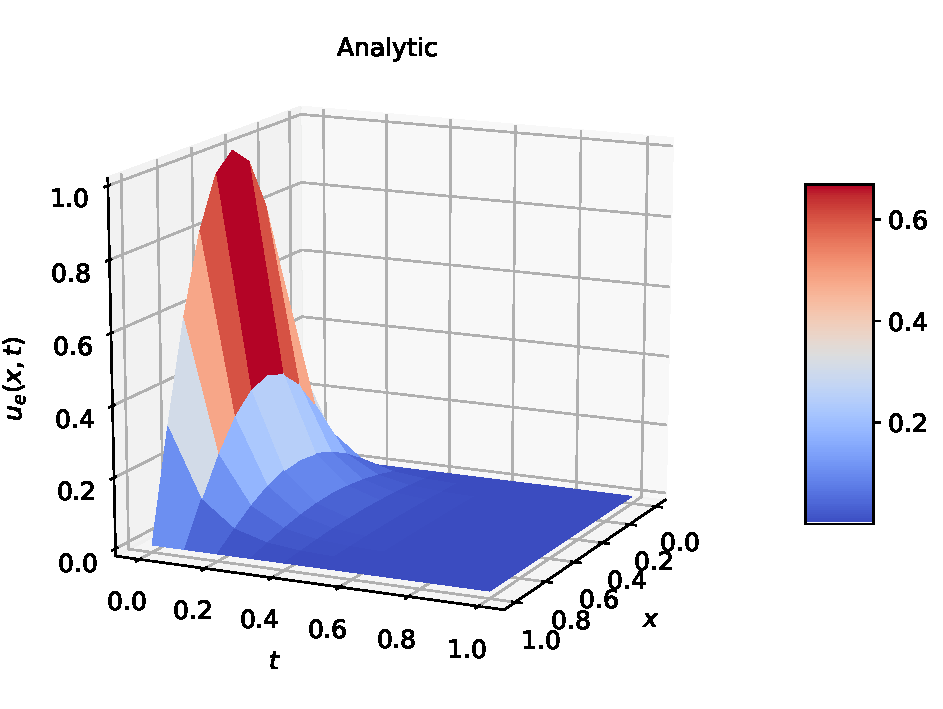
\includegraphics[scale=0.48]{latex/figures/heat_ana_nn3.pdf}}}
\qquad
\subfloat[]{{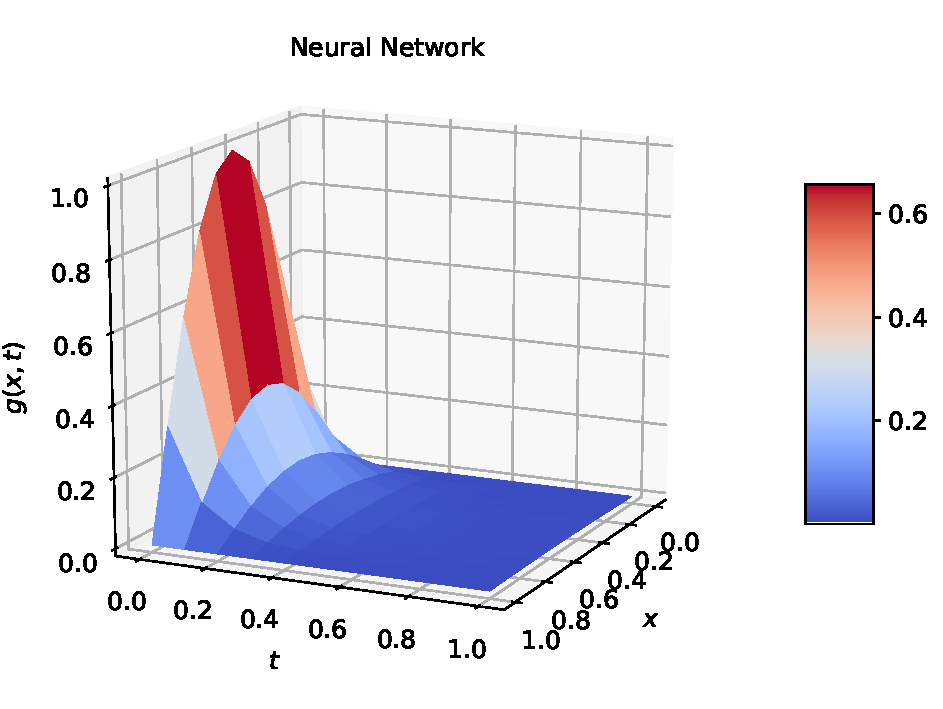
\includegraphics[scale=0.48]{latex/figures/heat_nn3.pdf}}}
\qquad
\subfloat[]{{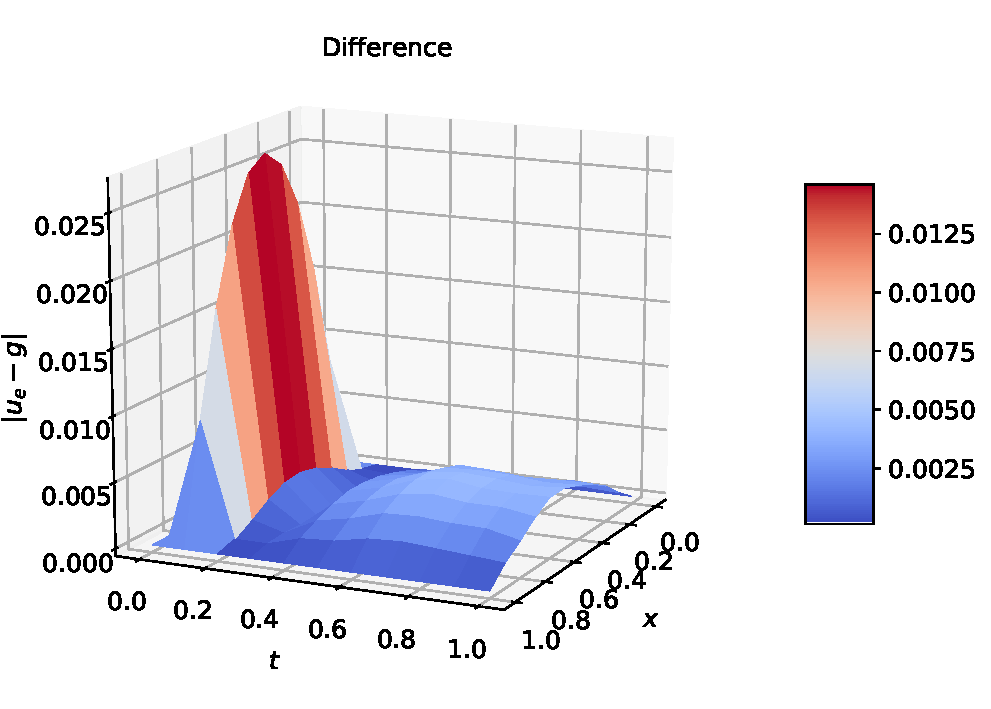
\includegraphics[scale=0.5]{latex/figures/heat_diff_nn3.pdf}}}
\caption{Model 2, Plot solution on the grid FFNN is trained on}
\label{fig:heat_nn3}
\end{figure}

\autoref{fig:heat_nn4} Plot solution on a larger grid than FFNN is trained on, i.e., points must be interpolated

301, 301 points

Max diff: 0.03215260678986426
Mean diff: 0.003950743671390742

\begin{figure}[H]
\centering
\subfloat[]{{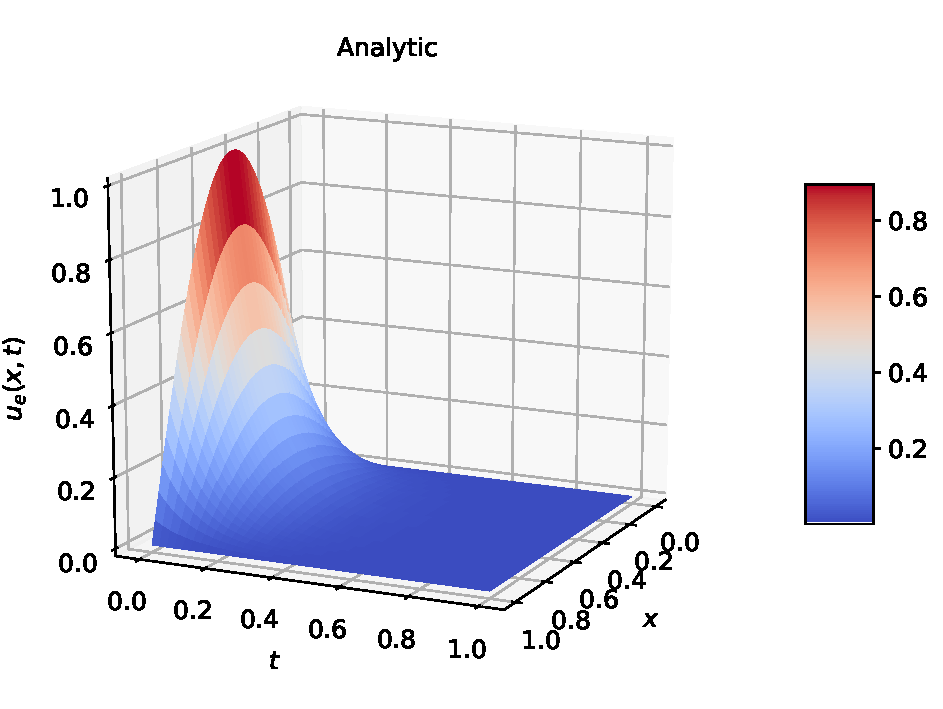
\includegraphics[scale=0.48]{latex/figures/heat_ana_nn4.pdf}}}
\qquad
\subfloat[]{{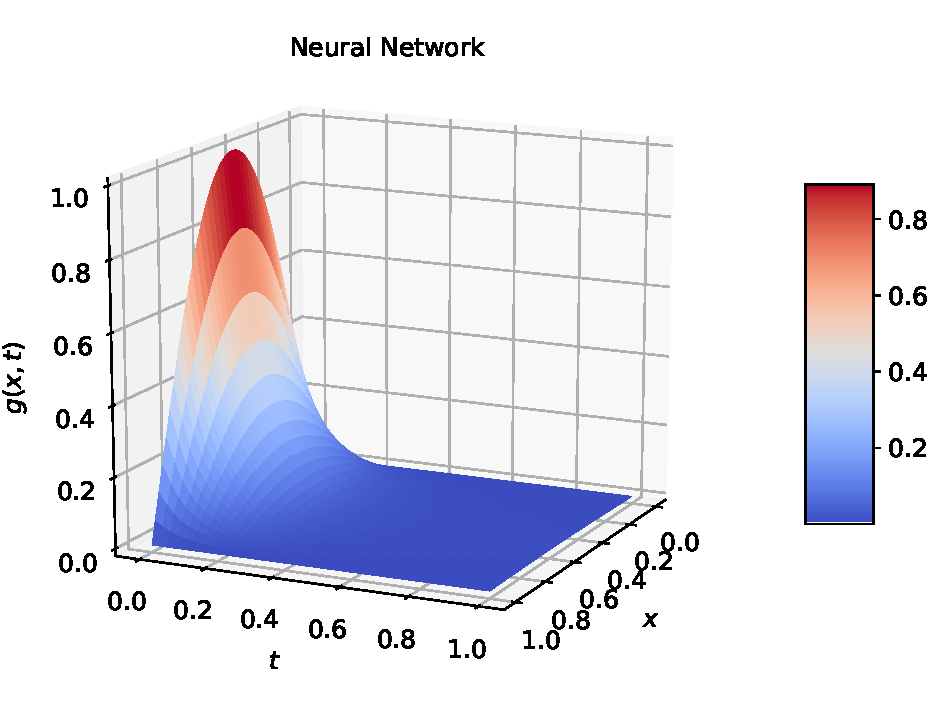
\includegraphics[scale=0.48]{latex/figures/heat_nn4.pdf}}}
\qquad
\subfloat[]{{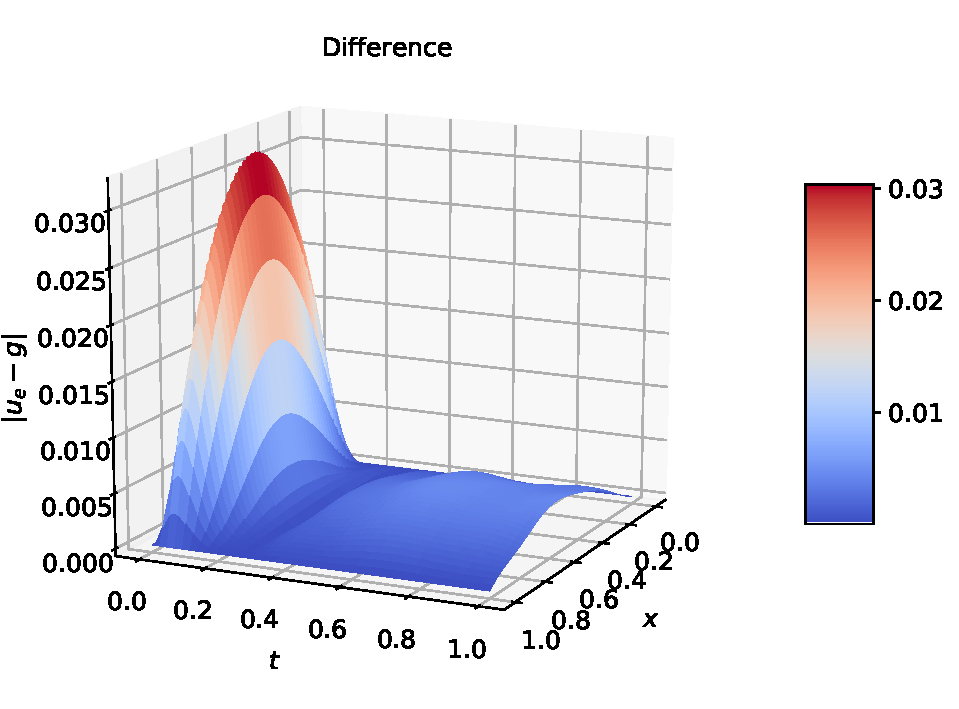
\includegraphics[scale=0.5]{latex/figures/heat_diff_nn4.pdf}}}
\caption{Model 2, Plot solution on a larger grid than FFNN is trained on, i.e., points must be interpolated}
\label{fig:heat_nn4}
\end{figure}

\subsubsection{Home-made}


%----------------------------------------------------------------
\subsection{Eigenvalue Problem}\label{sec:eigenvalue results}
%----------------------------------------------------------------

Accompanying notebook: 


\subsubsection*{Benchmark ODE rhs with Euler}

\autoref{fig:euler_benchmark}, ODE RHS, two alternatives, benchmark which gives best result with Euler's method. simulation, time $t\in [0, 5]$ with $N = 101$ number of timesteps

\begin{figure}[H]
\centering
\subfloat[]{{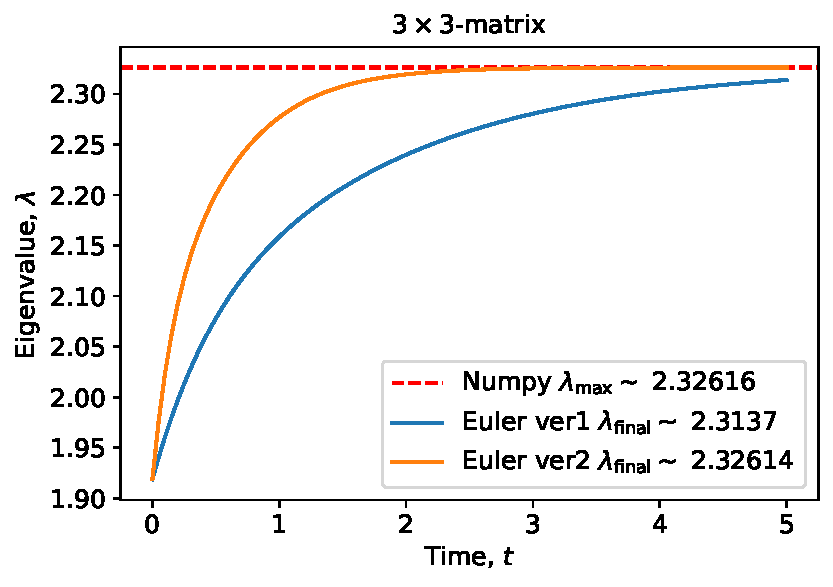
\includegraphics[scale=0.5]{latex/figures/euler_benchmark_33.pdf}}}
\qquad
\subfloat[]{{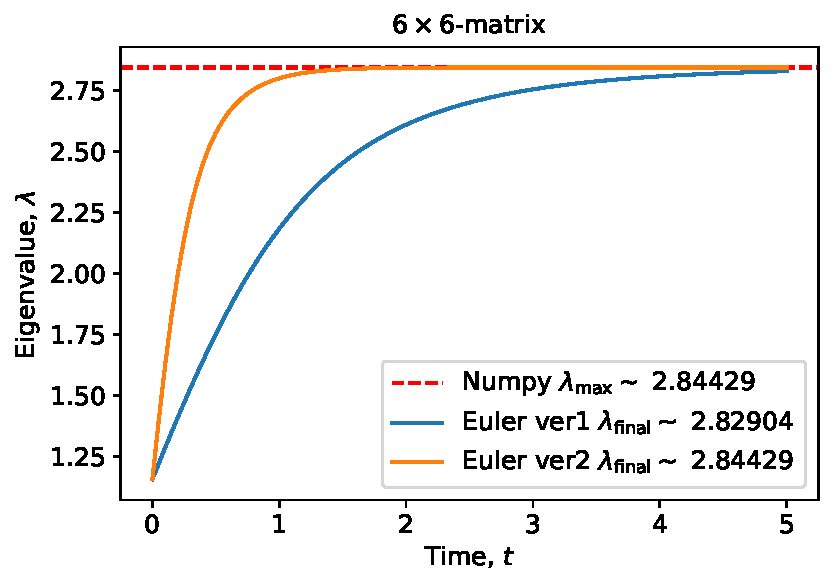
\includegraphics[scale=0.5]{latex/figures/euler_benchmark_66.pdf}}}
\caption{Euler's method with different expressions of the right-hand side of ODE (ref) tested on randomly generated real symmetric matrices; in \textbf{(a)} a $3\times 3$-matrix, and in \textbf{(b)} a $6\times 6$-matrix.}
\label{fig:euler_benchmark}
\end{figure}

From the figures it seems like ODE RHS ver1 converges somewhat slower than ver2 in the 3x3 case. In the 6x6 case, however, ver1 often struggles to converge as good as ver2 (multiple runs, which can be easily reproduced in jupyter notebook). Both these 'problems' probably arises because ver1 is more computationally demanding than ver2.

\subsubsection{FFNN, benchmark problem}

\begin{equation*}
    A = \left(\begin{array}{ccc}
        3 & 2 & 4  \\
        2 & 0 & 2  \\
        4 & 2 & 3
    \end{array}\right)
\end{equation*}
with eigenvalues $\lambda_1 = 8$ and $\lambda_2 = \lambda_3 = -1$.



\autoref{fig:benchrun1}; 3 layers + output [sigmoid, relu, sigmoid], [100, 50, 25]

Step: 1500, Loss: 0.014227586970184775

A = [[3. 2. 4.]
 [2. 0. 2.]
 [4. 2. 3.]]
x0 = [1 0 0]
Eigvals Numpy: [-1.  8. -1.]
Max Eigval Numpy 8.0
Final Eigval Euler 7.999999884131663
Final Eigval FFNN 7.999994245949094

\begin{figure}[H]
\centering
\subfloat[]{{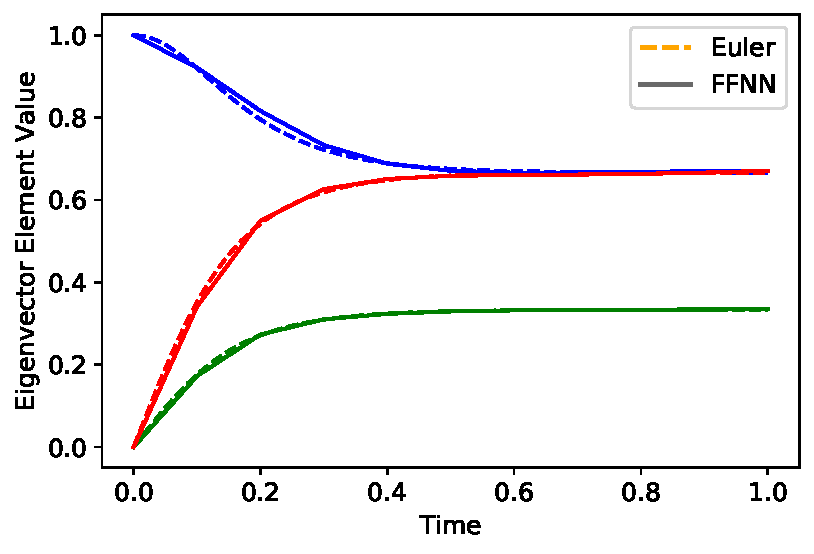
\includegraphics[scale=0.5]{latex/figures/eigvec_comp_benchrun1.pdf}}}
\qquad
\subfloat[]{{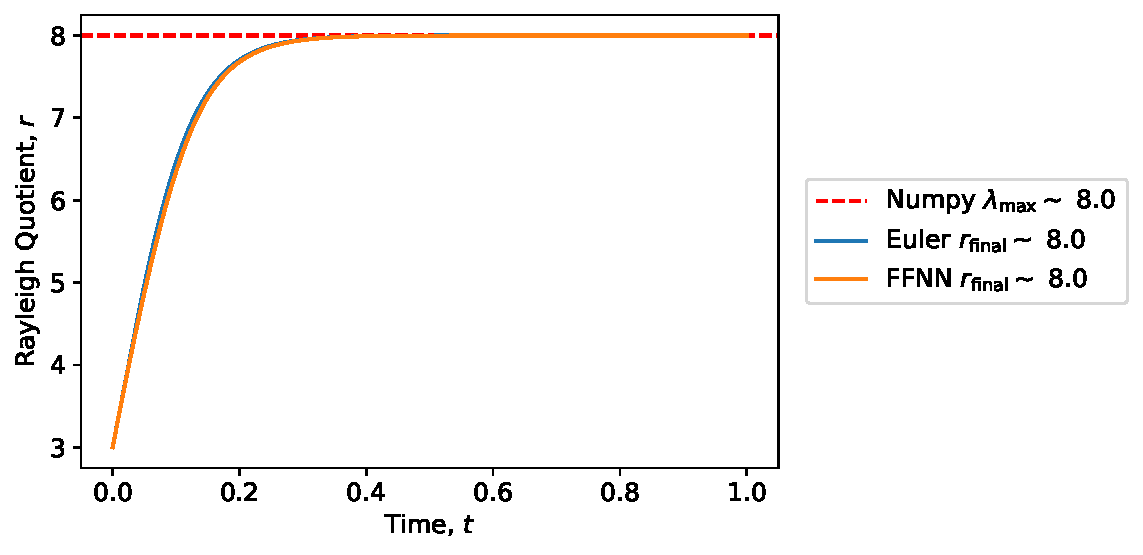
\includegraphics[scale=0.5]{latex/figures/eigval_benchrun1.pdf}}}
\caption{Benchrun 1 \textbf{(a)} Components of steady-state vector computed with both Euler's method (dashed lines) and the feed-forward neural network (solid line). \textbf{(b)} Computed maximum eigenvalue }
\label{fig:benchrun1}
\end{figure}

